
\chapter{Results}  \label{sec:results}


\section{Experiments}  \label{sec:experiments}

To evaluate the effectiveness of the previously defined \ac{dea}, a series of experiments are conducted using multiple datasets.
These experiments aim to assess the attack’s performance across different encoding schemes and dataset characteristics, and to analyze its ability to reconstruct plaintext information from encoded identifiers.

The primary dataset used is the \texttt{fakename} dataset, which is synthetically generated using the American name set provided by the Fake Name Generator.
This dataset was previously employed in related work by Schaefer et al.~\cite{schaefer2024}, making it a suitable benchmark for comparative evaluation.
It includes realistic combinations of personal identifiers and is well-suited for testing the scalability and reliability of both the \ac{gma} and \ac{dea} pipelines.

The \texttt{fakename} datasets consist of synthetically generated entries, each containing a given name, surname, and date of birth.
These datasets aim to resemble realistic combinations of personal identifiers while ensuring privacy and reproducibility.
For evaluation purposes, multiple dataset instances of varying sizes are used: 1{,}000, 2{,}000, 5{,}000, 10{,}000, 20{,}000, and 50{,}000 entries.

The primary advantage of using this dataset family lies in its scalability.
By maintaining a consistent schema while varying the number of records, the impact of dataset size on the performance and success of the \ac{dea} can be systematically analyzed.
This enables controlled experiments that highlight how the quantity of available data influences re-identification, training quality, and generalization performance of the attack models.

An additional dataset used in this study is the \texttt{euro\_person} dataset provided as part of the simulated data for the ESSnet DI on-the-job training course on record linkage, held in Southampton from 25--28 January 2011.
The dataset was created by Paula McLeod, Dick Heasman, and Ian Forbes from the UK Office for National Statistics and contains realistic, fictionalized personal information intended for the training and evaluation of record linkage techniques.
The \texttt{euro\_person} dataset includes forename (\texttt{PERNAME1}), surname (\texttt{PERNAME2}), and full date of birth composed of day, month, and year, which were concatenated into a single \texttt{DOB\_FULL} attribute for the purposes of this work.
The dataset consist of 26.625 records.
As the dataset also serves as a ground-truth reference for other simulated sources such as Census, CIS, and PRD, it is well-suited for evaluating the precision and completeness of plaintext reconstruction and re-identification in the context of the \ac{dea}.

In addition to the synthetic and benchmark datasets, this thesis also incorporates a curated version of the Titanic passenger manifest, referred to as \texttt{titanic\_full}.
This dataset consists of 891 unique records and includes the fields \texttt{firstname}, \texttt{surname}, and a numeric \texttt{uid} used for internal tracking.
While not originally intended for record linkage evaluation, the dataset offers a semi-realistic collection of personal identifiers derived from historical records.
It provides a useful test case for examining the impact of natural name diversity, varying name lengths, and non-standard naming formats (e.g., inclusion of titles or parenthetical information) on the performance of both Graph Matching and Dataset Extension Attacks.
Due to the historical and English centric nature of the data, it shares some limitations with other Western-focused datasets used in this work but nonetheless adds valuable variety in terms of name structure and frequency.

The experiments are conducted across a range of settings and scenarios to comprehensively evaluate the effectiveness of the \ac{dea}.
Each encoding scheme, namely \ac{bf}, \ac{tsh}, and \ac{tmh}, is tested individually across all datasets as described earlier.
This allows for a direct comparison of reconstruction performance under different privacy-preserving encoding mechanisms.

To additionally analyze how the quality of the training data affects the \ac{dea}, the preceding \ac{gma} step is executed with varying levels of overlap between Alice's and Eve's datasets.
For each dataset and encoding scheme, the \ac{gma} is run multiple times with overlap ratios ranging from 20\% to 80\%, in increments of 20\%.
This simulates different real world scenarios where the attacker has access to varying amounts of auxiliary information.
The resulting re-identifications from the \ac{gma} then serve as the labeled training data for the \ac{dea}, thus allowing for a detailed evaluation of how overlap levels influence overall reconstruction success.

In addition to varying dataset sizes and overlap levels, different attacker scenarios are considered to evaluate the robustness of the \ac{dea} under more and less realistic assumptions.
The first scenario, Eve's auxiliary dataset $D_e$ is a strict subset of Alice's dataset $D_p$, i.e., $D_e \subseteq D_p$.
In this case, the overlap $o$ is defined as the ratio $o = \frac{|D_e|}{|D_p|}$.
The elements in $D_e$ are generated by randomly sampling $|D_e| = \lfloor o \cdot |D_p| \rfloor$ records from $D_p$ without replacement.
While this setup simplifies evaluation and isolates the impact of training data availability, it is also highly idealized and does not reflect the complexity of real world linkage scenarios.

To address this, a second, more realistic setting is also considered, where both $D_p$ and $D_e$ contain disjoint as well as overlapping individuals.
That is, $D_e \nsubseteq D_p$, but $D_e \cap D_p \neq \emptyset$.
In this scenario, the auxiliary and target datasets each include individuals not present in the other, simulating cases where Eve has partial but non exclusive knowledge of the data.
This setup introduces additional challenges for both the \ac{gma} and \ac{dea}, as structural mismatches and auxiliary noise may degrade re-identification and reconstruction accuracy.

This setup mirrors the experimental methodology employed by \cite{schaefer2024}, ensuring consistency and comparability with prior work on the \ac{gma}.
By varying the overlap rate and dataset composition in this way, a diverse range of re-identification scenarios is created, which directly impacts the amount and quality of training data available for the \ac{dea}.
This, in turn, enables a systematic evaluation of the \ac{dea}'s ability to generalize from partially re-identified data.
As the \ac{gma} identifies different subsets of individuals under varying overlap conditions, the resulting re-identification sets are used to train the neural network, while the remaining non matched records serve as the test set.
Thus, each experiment yields a distinct train-test split, providing a rich basis for assessing the reconstruction capabilities of the \ac{dea} under different supervision levels and graph-matching outcomes.

For the \ac{dea} specific configuration, several fixed settings were employed to ensure comparability across all experimental conditions.
First, the dataset of re-identified individuals, used as labeled training data, was split into training and validation sets using a fixed 80/20 ratio.
This choice reflects common machine learning practice and provides a balanced compromise between model learning and validation reliability.

One of the most critical components of the \ac{dea} pipeline is the hyperparameter optimization step, which is responsible for identifying the most effective neural network architecture.
For this purpose, a total of 125 trials were conducted for each experimental setting.
This number was chosen to provide sufficient coverage of the hyperparameter space while maintaining computational feasibility.

Each trial, as well as the final training run for the best performing model, was limited to a maximum of 20 training epochs.
While this represents a relatively high upper bound, overfitting is mitigated through the use of early stopping.
Specifically, training was halted if the validation loss did not improve for five consecutive epochs (patience = 5), with a minimum delta of $1 \cdot 10^{-4}$ required to qualify as an improvement.
This strategy ensures both efficient training and effective model selection, especially when performance plateaus early.

The search space for the hyperparameter optimization follows the configuration described in Section~\ref{sec:hmo}.
Throughout the entire \ac{dea} pipeline, the \textbf{Dice coefficient} is used as the objective metric for optimization.
This choice is motivated by its robustness and balanced nature, as it integrates both precision and recall and has consistently yielded the most promising results during preliminary manual testing.

For efficient optimization, the hyperparameter search is executed using $n - 1$ CPU cores, where n is the number of available logical processors.
This allows for near maximal parallelism during hyperparameter tuning, significantly reducing the total runtime without compromising system stability.

In the final re-identification phase, two reconstruction strategies are evaluated to enable comparative analysis: (1) the greedy, graph-based reconstruction method described in Section~\ref{sec:graphrecon}, and (2) the dictionary-based fuzzy matching approach described in Section~\ref{sec:dictrecon}.
Both methods are deterministic and computationally efficient, making them suitable for large scale experimental evaluation.

The language model based reconstruction method is deliberately excluded from the evaluation.
Despite showing potential in early qualitative testing, its dependence on proprietary models, token-based pricing, and limited reproducibility make it unsuitable for scalable and reproducible experimentation within the current research setting.

All experiments were conducted on a virtual machine running Ubuntu 22.04, equipped with 22 cores of an AMD EPYC 9254 processor.
The system was provisioned with 435\,GB of DDR5 RAM and featured an NVIDIA GeForce RTX 3090 Ti GPU with 24\,GB of dedicated VRAM.

This high-performance computing setup enabled efficient parallel execution of the hyperparameter optimization trials and accelerated training of the neural networks via GPU.
The extensive memory capacity was particularly beneficial during dataset preprocessing and batch-wise loading of large datasets, ensuring that all encoding schemes and reconstruction strategies could be evaluated without resource bottlenecks.

\section{Evaluation Metrics}  \label{sec:metrics}

The performance of the \ac{dea} is assessed using several metrics that are systematically recorded throughout the experimental runs.

Although the \ac{dea} constitutes an offline attack, meaning the adversary can operate without time constraints once both encoded datasets are available, the runtime of the attack remains a valuable indicator of its practical feasibility.
Therefore, the total runtime as well as the runtime of each individual stage within the \ac{dea} pipeline (e.g., data preprocessing, model training, inference, and reconstruction) is measured and documented.

A central metric for assessing the effectiveness of the attack is the \emph{re-identification rate}.
This metric is defined as the number of individuals that are successfully and correctly re-identified by the \ac{dea}, divided by the total number of individuals who were not matched during the initial \ac{gma}.
A successful re-identification in this context means that the \ac{dea} is able to fully reconstruct the original plaintext attributes of a record such that it exactly matches a record in Alice's encoded dataset.
Thus, the re-identification rate reflects the proportion of previously unmapped individuals that the attacker can recover using the inference based approach.

Another important aspect of evaluating the \ac{dea} is its performance in predicting the correct n-grams, which form the basis for reconstructing plaintext attributes.
To assess the quality of these predictions, several standard classification metrics are considered—namely, \textbf{precision}, \textbf{recall}, and the \textbf{F1-score}.

Precision measures the proportion of correctly predicted n-grams among all predicted n-grams, thereby quantifying the model’s ability to avoid false positives.
Recall, on the other hand, captures the proportion of true n-grams that were successfully recovered, reflecting the completeness of the reconstruction.
The F1-score, which is the harmonic mean of precision and recall, offers a balanced assessment of the model's correctness and coverage.

In the context of this work, the F1-score is of particular interest, as it has shown to be the most reliable metric for quantifying n-gram-level performance.
Moreover, it is mathematically equivalent to the Dice similarity coefficient for binary sets, making it not only interpretable but also consistent with the optimization objective used during the hyperparameter tuning stage (cf. Section~\ref{sec:experiments}).
This alignment ensures that the evaluation metric reflects the actual optimization goal of the \ac{dea}.

To enable a meaningful comparison, the performance of different \ac{dea} configurations is evaluated not only against each other but also against a baseline strategy.
This baseline serves as a lower bound for the expected prediction quality and helps contextualize the improvements achieved through the proposed neural reconstruction pipeline.

The baseline approach simulates an attacker who, for each non re-identified individual, simply predicts the most frequent n-grams across the entire dataset.
This assumes that the attacker has full access to the distribution of n-grams in the encoded dataset, a reasonable assumption in a research setting, where the dataset is known, but less realistic in real-world attacks.
Still, it provides a practical lower-bound for evaluation.

An analysis of the \texttt{fakename} datasets revealed that the average total length of a full entry, comprising first name, surname, and date of birth, is approximately 21 characters.
Given that 2-grams are used for encoding, this corresponds to roughly 20 overlapping 2-grams per entry.
Consequently, the baseline is defined by selecting the top $k=20$ most frequent 2-grams across the entire dataset and predicting this fixed set for every test record.
This naive method disregards any record specific characteristics and instead reflects a population wide frequency-based guess, serving as a simple yet informative lower bound for comparison.

The result is a dataset specific set of baseline metrics, precision, recall, F1-score, and Dice similarity, against which the \ac{dea} model's predictions can be compared.
These baseline metrics vary with dataset size, since the n-gram frequency distribution shifts with the number of records.
The aggregated results of the baseline performance across datasets are visualized in Figure~\ref{fig:baseline_metrics}.


\begin{figure}[H]
    \centering
    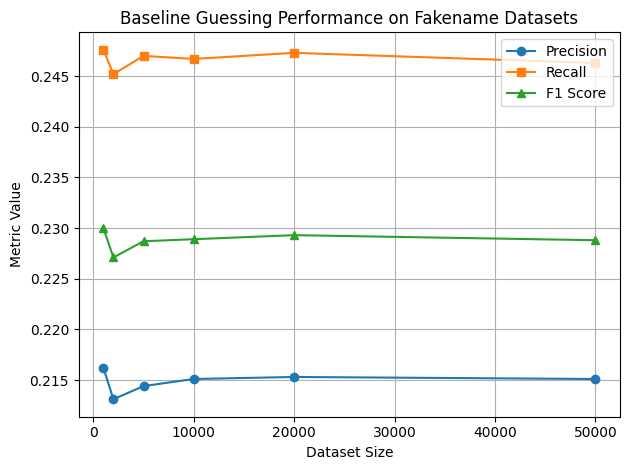
\includegraphics[width=0.7\textwidth]{img/fakename_analysis.png}
    \caption{Evaluation of the baseline performance on the \texttt{fakename} dataset: For each dataset size, the prediction quality of the 20 most frequent 2-grams is shown in terms of \textbf{precision}, \textbf{recall}, and \textbf{F1-score}. The average entry length is 21 characters.}
    \label{fig:baseline_metrics}
\end{figure}

For the \texttt{euro\_person} dataset, the baseline strategy for evaluating the effectiveness of the \ac{dea} follows the same procedure as for the \texttt{fakename} dataset.
Specifically, the most frequent n-grams in the training data are used to simulate a naïve guessing approach.
Based on the analysis of this dataset, the average length of a full entry, comprising forename, surname, and full date of birth, is approximately 20 characters.
Assuming the use of 2-grams with overlapping character windows, this corresponds to around 19 distinct 2-grams per entry.

As a baseline, the top 19 most frequent 2-grams are selected and uniformly predicted for each record, independent of the individual characteristics of the entries.
This approach mirrors a realistic but simplistic attacker model, who relies solely on population-level frequency statistics without individual-level inference.

The resulting performance metrics for this baseline prediction indicate a precision of 0.2197, a recall of 0.2446, and an F1-score of 0.2306.
These values provide an important reference point for evaluating the added value of the \ac{dea} pipeline, as they quantify the effectiveness of a purely frequency driven reconstruction approach.

For the \texttt{titanic\_full} dataset, a frequency-based baseline was used to assess the difficulty of reconstructing full identifiers from predicted n-grams.
The average length of a full entry (consisting of given name and surname) in this dataset is approximately 26 characters, indicating relatively high complexity due to longer and often multi-token names.
The baseline reconstruction approach achieved a precision of 0.2468, a recall of 0.3770, and an F1 score of 0.2896.
These modest performance values reflect the structural challenges posed by the dataset, including the presence of honorifics, compound names, and non-standard formatting.
The results suggest that even a naïve guessing strategy can partially recover plaintext identifiers, but also establish a meaningful lower bound for evaluating the performance improvements of learning-based approaches such as the Dataset Extension Attack.

Notably, for the \texttt{titanic\_full} dataset, the overlap ratio used in the experiments was adjusted to the set \{0.2, 0.4, 0.6, 0.7, 0.8, 0.9\}.
This adaptation was necessary because the dataset is relatively small, and the \ac{gma} fails to identify any individuals at lower overlap values.
Meaningful results only begin to emerge at an overlap of 0.7 or higher.

Notably, the similarity of the baseline metrics to those obtained on the \texttt{fakename} dataset highlights the generality of the method across synthetic and semi-realistic datasets, further justifying its inclusion as a comparative benchmark.

\section{Analysis}  \label{sec:analysis}

In this section the results of the \ac{dea} experiments are presented and analyzed.
The analysis is structured into several subsections, each focusing on a specific aspect of the \ac{dea} performance.
As described in Section~\ref{sec:experiments}, the experiments were conducted across multiple datasets, encoding schemes, overlaps and drop from settings.
Therefore, several of these configuration settings will be fixed to analyze the impact of the remaining parameters on the \ac{dea} performance.

One important aspect especially for smaller datasets and overlap sizes is, that it could occur that the \ac{gma} does not identify any individuals, i.e., the re-identification set is empty.
In this case, the \ac{dea} is not able to reconstruct any plaintext information.
This is the case because if there are no re-identified individuals in place, there is no training data for the \ac{dea} available.
Therefore the results of these experiments are not reported and the corresponding data points are excluded from the analysis and plots.

\subsection{\ac{tmh}}

The following subsection is going to focus on the results obtained using the \ac{tmh} encoding scheme.
For the following analysis, each dataset is evaluated under different aspects.
Therefore the dataset will be fixed and the analysis will focus on the different results vor varying overlap sized ans drop from strategies.

\paragraph{Titanic Full}

The DEA using TabMinHash encoding achieves strong F1 scores on the Titanic dataset, with a peak of 0.76 for \texttt{DropFrom = Eve} and 0.68 for \texttt{DropFrom = Both} at overlap 0.9.
This performance is largely driven by high precision (above 0.9) and improved recall, especially for Eve at 0.8 overlap (0.64).
Compared to lower-overlap settings, the model benefits significantly from greater data redundancy.
While Both initially underperforms Eve at 0.7–0.8, the gap narrows at higher overlap values.

As with the Bloom Filter encoding, no successful re-identifications are observed—neither fuzzy nor greedy matchers identify any records across overlaps.
Despite solid structural learning, the model remains ineffective at linking back to individual identities on this dataset.

Runtime remains low (under 10 minutes), with Eve consistently faster than Both. The HypOp validation scores slightly underestimate the full-data F1, but overall tracking is close, particularly at higher overlaps.

In summary, TabMinHash performs well on the Titanic dataset in terms of predictive accuracy, but—like its Bloom Filter counterpart—fails to achieve individual re-identification under the evaluated conditions.


\paragraph{Fakename 1k}
The DEA evaluation on the TabMinHash encoding for the fakename 1k dataset reveals several noteworthy trends.
When using the \texttt{DropFrom = Eve} configuration, the DEA consistently outperforms the baseline F1 score for overlaps higher than 0.4.
Specifically, at overlaps of 0.6 and 0.8, the trained F1 score reaches approximately 0.54 and 0.58 respectively, clearly surpassing the baseline of around 0.2.
This improvement is also reflected in the recall, which increases from about 0.11 at 0.4 overlap to over 0.42 at 0.8.
Precision remains consistently high for Eve (above 0.95 across all overlaps), indicating that while not all matches are found, those that are predicted are likely correct.
In contrast, the \texttt{DropFrom = Both} configuration exhibits significantly weaker performance, only approaching the baseline F1 at the highest overlap (0.8), with notably lower recall and precision in all other settings.
Interesting is the spike of precision at 0.8 overlap to nearly 0.9.

Despite the promising F1 scores, the actual re-identification rate remains at 0\% across all overlaps and drop strategies.
None of the applied re-identification methods (greedy, fuzzy, or their combination) could recover any individual's true identity, indicating that while the model learns statistical patterns, it does not enable perfect linkage to plaintext identities.

In terms of runtime, the Eve strategy incurs a higher computational cost, particularly at 0.6 overlap (about 16 minutes), compared to the Both strategy, which remains under 14 minutes.

However, this tradeoff is justified by the significantly improved performance.
Additionally, when comparing trained F1 scores against validation F1 (HypOp), all points lie below the $x = y$ line, suggesting that the full model generalizes better than indicated during validation.
This underestimation highlights that the HypOp metric may be conservative and not fully reflect the model’s potential when applied to the entire dataset again.

Overall, these results show that the DEA can exploit structural patterns in TabMinHash encodings effectively when Eve is the only source of missing entries and overlap is sufficiently high.
However, the inability to re-identify individuals directly suggests that while aggregate information can be extracted, privacy at the individual level is maintained under these conditions.

\paragraph{Fakename 2k}

Compared to the 1k dataset, the DEA performance on the 2k version shows even clearer improvements when using \texttt{DropFrom = Eve}.
At overlaps of 0.6 and 0.8, the trained F1 reaches 0.58 and 0.72 respectively, again clearly surpassing the baseline.
Recall increases substantially (up to 0.61 at 0.8), and precision remains high (>0.9) except for a dip at 0.6.
In contrast, the \texttt{DropFrom = Both} strategy performs poorly across all metrics, with only marginal gains in F1 and recall.

Similar to the 1k case, the re-identification rate remains 0\% for all overlap levels and matching methods, reaffirming that the model exploits structural patterns but fails to link any record back to its plaintext identity.
The runtime for the Eve configuration is surprisingly lower than for Both, despite stronger performance.
The generalization gap observed in the \texttt{HypOp vs. Full F1} plot persists, with trained performance consistently exceeding validation scores.

Overall, the trend confirms that increasing dataset size and overlap improves DEA effectiveness under the Eve setting, while direct re-identification remains infeasible.

\paragraph{Fakename 5k}

With the larger fakename 5k dataset, the DEA achieves its strongest results so far, especially for \texttt{DropFrom = Eve}.
F1 peaks at 0.87 for overlap 0.6 and remains above 0.7 across higher overlaps.
Precision nearly saturates at 1.0, while recall reaches 0.79.
Compared to the 1k and 2k datasets, both the quality and stability of predictions improve significantly.
Even the \texttt{DropFrom = Both} configuration becomes effective, surpassing the baseline for overlaps $\geq$ 0.6.

For the first time, a small number of re-identifications occur: up to 1.2\% (Eve) and 0.01\% (Both) at overlap 0.6.
These are still rare, but mark a turning point in the attack’s ability to directly reconstruct individuals.
Runtime increases substantially with dataset size, peaking around 74 minutes.
The validation F1 (HypOp) continues to underestimate final performance, though the gap is narrower than in smaller datasets.

These results indicate that with sufficient data volume and overlap, the DEA begins to break through into direct re-identification territory, especially when only Eve’s side is incomplete.

\paragraph{Fakename 10k}
With 10{,}000 records, the DEA reaches peak performance.
For \texttt{DropFrom = Eve}, the trained F1 climbs above 0.9 (overlap $\geq$ 0.6), and recall reaches 0.91, far exceeding the baseline.
Precision saturates at nearly 1.0 across both drop strategies.
Notably, \texttt{DropFrom = Both} also becomes effective with increasing overlap, achieving an F1 of 0.9 at overlap 0.8.
Compared to the 5k dataset, all metrics improve further in both quality and consistency.

Importantly, re-identification becomes significant: up to 5.3\% for Eve and 2.9\% for Both at overlap 0.8, marking the first clear success in reconstructing individual identities.
Greedy and fuzzy matching both contribute, with the combined method performing best.
Runtime grows substantially, reaching up to 170 minutes, reflecting the scaling cost of training.
As in previous experiments, the validation F1 underestimates final performance, though the top points begin to approach the $x = y$ line.

Overall, this setting shows that the DEA not only recovers accurate group-level patterns but now also breaches individual privacy when data size and overlap are high.

\paragraph{Fakename 20k}

On the largest dataset so far, the DEA reaches its highest effectiveness.
Trained F1 exceeds 0.9 for both \texttt{DropFrom = Eve} and \texttt{DropFrom = Both} at overlap 0.8.
Recall remains above 0.9 for Eve and 0.86 for Both, with near-perfect precision across all settings.
Unlike smaller datasets, the Both strategy now reliably outperforms the baseline, even at lower overlap, —demonstrating that DEA benefits from both increased data volume and redundancy.

Re-identification becomes alarmingly effective: Eve enables recovery of up to 13.2\% of individuals at overlap 0.8, while Both yields up to 10.2\%.
The gap between matching strategies is consistent across all dataset sizes—\emph{greedy} matching always outperforms \emph{fuzzy}, indicating that more confident matches based on exact substring positions are more successful.

Runtime increases substantially, exceeding 350 minutes in some cases, which aligns with the observed pattern of increasing compute cost with dataset size.
The generalization gap between validation and full data F1 narrows for high-performing runs, but underfitting remains visible at lower overlaps.

In summary, at 20k records, the DEA no longer just learns structure, it reliably performs direct re-identification.
The attack is most effective under the Eve strategy with high overlap, but Both is no longer a safe configuration as well.

\paragraph{Europerson}

For the euro person dataset, the DEA again achieves strong results across all overlaps and configurations.
Trained F1 scores are consistently high, peaking at 0.95 for both \texttt{DropFrom = Eve} and \texttt{Both}, significantly above the baseline.
Recall and precision also remain high across all settings, suggesting stable and reliable model behavior.
Unlike the fakename datasets, the Both strategy performs comparably well or even slightly better than Eve in terms of F1, indicating that the model generalizes robustly even when information is dropped symmetrically.

Re-identification is effective but concentrated at overlap 0.6, reaching 6.7\% for Both and 6.1\% for Eve.
As in previous datasets, \emph{greedy} matching consistently outperforms \emph{fuzzy}.
This reaffirms earlier observations that greedy matching is more effective for this task.
The drop in re-ID rates at overlap 0.8, despite high model performance, suggests potential saturation effects or ambiguity in the match space.

Training times exceed 400 minutes in some cases, continuing the trend of exponential runtime growth with dataset complexity and size.
However, the \texttt{HypOp vs. Full F1} plot shows nearly perfect correlation, suggesting excellent validation accuracy and minimal overfitting—marking a notable improvement over previous runs.

In summary, the DEA remains highly effective on the euro person dataset, with robust re-identification capabilities and strong generalization, especially under symmetric drop scenarios.


\subsection{\ac{tsh}}

\paragraph{Titanic Full}

The TwoStepHash encoding yields consistently strong DEA performance on the Titanic dataset.
F1 scores steadily increase with overlap, reaching 0.79 for \texttt{DropFrom = Eve} and 0.80 for \texttt{DropFrom = Both} at 0.9 overlap.
This balanced performance across both configurations is supported by high precision values—above 0.95 for Both—and recall values climbing to over 0.74.
Unlike TabMinHash, which favored Eve at lower overlaps, TwoStepHash appears more stable and symmetric in terms of learned patterns.

Despite the good predictive performance, re-identification remains unsuccessful: no matches are found using fuzzy or greedy strategies, indicating that while structural properties are recoverable, they do not yet support direct identity resolution under these conditions.

Training times are moderate, ranging from 9 to 14 minutes, and the HypOp F1 scores closely follow the final results—indicating effective model selection.
The validation-to-full F1 correlation is especially tight at higher overlaps, with only a minor underestimation in one configuration.

In conclusion, TwoStepHash performs reliably on the Titanic dataset, yielding high-precision reconstructions but no re-identifications—similar in privacy behavior to the other encoding methods tested.


\subsection{\ac{bf}}

\paragraph{Titanic Full}

The DEA achieves high trained F1 scores on the Titanic dataset, peaking at 0.83 for \texttt{DropFrom = Both} and 0.81 for \texttt{DropFrom = Eve} at overlap 0.8.
Precision and recall both exceed 0.9 and 0.7 respectively in these top-performing settings, indicating that the model successfully captures structural patterns from Bloom Filter encodings.
Compared to other datasets, performance is already strong at relatively high overlaps (0.7–0.9), and Both performs equally well or slightly better than Eve, suggesting that sufficient redundancy exists even under symmetric dropout.

Despite strong classification results, no successful re-identifications are observed across any setting.
Both fuzzy and greedy matching produce 0\% re-ID rates, showing that although the model generalizes well, it does not achieve individual-level deanonymization on this dataset.

Training times remain short, ranging from 6.8 to 9.1 minutes, and validation scores closely match full-data F1—indicating well-calibrated HypOp selection.
Overall, while the model effectively learns link structures in the Titanic data, it falls short of re-identification, likely due to the dataset’s size and feature variability.


\paragraph{Fakename 1k}

On the fakename 1k dataset, the DEA using Bloom Filter encoding begins to show effective learning behavior under the \texttt{DropFrom = Eve} setting.
The trained F1 score improves significantly with overlap, reaching 0.68 at 0.8, far above the baseline.
This increase is driven by a steady rise in recall (from 0.04 to 0.53) and consistently high precision (up to 0.93).
In contrast, the \texttt{DropFrom = Both} configuration fails to show meaningful improvements, with F1 scores plateauing below 0.2 and recall staying low despite overlap increases.

Despite strong F1 gains, no successful re-identifications are observed across any configuration or overlap.
Both greedy and fuzzy matching yield 0\% re-ID rates, indicating that while the model captures structural information, it cannot yet link encoded entries to plaintext identities.
Runtime peaks at 19 minutes for Eve at 0.6 overlap and remains manageable throughout.

The validation F1 (HypOp) underestimates full-data performance, especially for higher overlaps, consistent with trends seen in early-stage DEA setups.
In summary, the Bloom Filter DEA on the 1k dataset demonstrates its first signs of structural reconstruction under Eve-only dropout, though without successful individual-level re-identification.

\paragraph{Fakename 2k}

With 2{,}000 records, the DEA shows marked improvements over the 1k setup, especially for \texttt{DropFrom = Eve}.
The trained F1 rises sharply with overlap, reaching 0.86 at 0.8.
Recall increases to 0.8, and precision remains above 0.9, showing the model's growing capacity to identify correct patterns in Bloom Filter encodings.
In comparison, the \texttt{DropFrom = Both} strategy improves slightly but remains less effective, with F1 peaking at 0.72 and lower recall across all overlaps.

For the first time, successful re-identifications occur: up to 1.5\% for Eve and 0.3\% for Both at overlap 0.8.
As observed earlier, \emph{greedy} matching begins to outperform \emph{fuzzy} as overlap increases, indicating stronger exact-match signals within the learned representations.

Runtime increases modestly, with Eve reaching nearly 40 minutes.
The HypOp metric still slightly underestimates final F1, but the gap narrows compared to the 1k dataset.
Overall, the model transitions from pattern learning to early-stage identity reconstruction, particularly under asymmetric dropout and high overlap.


\paragraph{Fakename 5k}

On the 5{,}000-record dataset, the DEA shows strong and increasingly stable performance.
Trained F1 peaks at 0.93 for \texttt{DropFrom = Eve} and 0.91 for \texttt{Both}, both at overlap 0.6, significantly higher than in the 2k setting.
Precision approaches 0.98–0.99, and recall exceeds 0.85, confirming the model's ability to learn accurate link structures from Bloom Filter encodings.
Interestingly, at overlap 0.8, performance slightly drops for Eve, while Both remains stable, suggesting that excessive overlap might reduce contrast for learning.

Re-identification becomes meaningful: the Eve strategy yields up to 5.1\% at overlap 0.6, and Both up to 1.6\%.
The dominant share of successful re-IDs again comes from \emph{greedy} matching, confirming its higher effectiveness over \emph{fuzzy}.
These findings mark the transition from merely reconstructing structure to reliably mapping individual identities.

Runtime increases to nearly 100 minutes in the Eve case, but remains manageable for Both.
As with earlier datasets, the HypOp validation score slightly underestimates final F1, though the correlation improves—especially for high-performing overlaps.

Overall, the 5k setting marks the first consistently successful phase of both structural learning and individual re-identification across dropout strategies.


\paragraph{Fakename 10k}

With 10{,}000 records, the DEA continues to scale effectively.
Trained F1 scores reach 0.94 for \texttt{DropFrom = Eve} and 0.91 for \texttt{Both} at overlap 0.6, confirming stable structural learning across both asymmetric and symmetric dropout settings.
Recall and precision remain very high (above 0.9) in all top-performing configurations.
Performance slightly drops at overlap 0.8, indicating potential over-saturation in the match space.

Re-identification becomes substantial: Eve yields a combined re-ID rate of 11.1\% and Both up to 7.9\% at overlap 0.6.
As in earlier datasets, \emph{greedy} matching consistently outperforms \emph{fuzzy}, with both contributing to the combined rate.
This confirms the dominance of greedy strategies in reliably identifying true matches in Bloom filter space.
Interestingly, re-ID performance dips again at 0.8 overlap, despite high F1—suggesting increased ambiguity among highly similar records.

Runtime grows further, with Both exceeding 150 minutes at overlap 0.2 and Eve remaining around 110 minutes at high overlap.
Validation F1 (HypOp) aligns closely with final results in high-performing runs, while low-overlap settings still show significant underestimation.

In summary, the 10k setting demonstrates mature DEA capabilities on Bloom Filters: both structure and identity are increasingly recovered, with Eve offering the highest success rates under intermediate overlap conditions.

\subsection{Comparison between Encoding Schemes}






% \subsection{DEA Complementing GMA}
% - Show how many additional re-identifications DEA achieved beyond GMA
% - Analyze overlap of DEA success with GMA failures
% - Visualize this improvement (e.g., stacked bar plot, Venn diagram)

% \subsection{Perfect Re-identification Rate}
% - Quantify the percentage of individuals that were fully reconstructed (i.e., all n-grams correct)
% - Compare across dataset sizes, overlap settings, and encodings
% - Relate full reconstructions to real-world identifiability

% \subsection{Performance Compared to Baseline}
% - Compare DEA vs. frequency-based guessing across precision, recall, F1
% - Emphasize improvements especially in precision or F1
% - Discuss whether the improvements are practically meaningful
% - Optional: show detailed comparison plots or tables


\section{Discussion}  \label{sec:discussion}


\subsection{Methodological Considerations and Setup Validity}
% - Suitability of datasets: fakename (controlled), euro_person (realistic)
% - Encoding scheme differences (BF, TSH, TMH)
% - Variability from GMA output affecting DEA

\subsection{Interpretation of Results}
% - DEA is helpful even when GMA fails (partial ground truth is enough)
% - High precision enables human inference, even when recall is low
% - Full reconstructions are not always necessary for privacy compromise

\subsection{Limitations and Practical Usefulness}
% - Results are based on synthetic or simulated data; real-world noise is higher
% - DEA results may not scale linearly with larger real-world datasets
% - The LLM-based reconstructor was omitted due to cost—but could outperform the others

\subsection{Comparison with Other Approaches}
% - GMA only works on overlapping individuals—DEA generalizes beyond
% - Traditional probabilistic record linkage lacks the capability for inference
% - Compare to adversarial learning, hill climbing, or brute-force attacks if applicable





